    \chapter{Convolutional Neural Network} \label{chap:cnn}
A \acrfull{cnn} is a type of \acrlong{nn} that is specialized in analyzing visual imagery. It has shown explemplary performance on serveral competitions related to Computer Vision and Image Processing \cite{khan_survey_2020}. \newline \newline
The first section introduces the building blocks of a \acrshort{cnn}. We start from the first and most simple element and then show the improvements. \newline \newline
The second section is concentrated on the training of a \acrshort{cnn}. \newline \newline
The third section details various models and techniques to perform model compression.
%%%%%%%%%%%%%%%%
    \section{Layers}
A layer is a high-level build block in \acrshort{dl}. It is a set of operations, weights and non-linear functions. It transforms an input into an output which will be used as input for another layer. The collections of layer is then used to build a \acrlong{cnn}. We begin our understanding of the layer theory by explaining the perceptron, the simplest element of a neural Network.
%%%
    \subsection{Perceptron} \label{subs:perceptron}
    \subsection{Perceptron} \label{subs:perceptron}
The perceptron was first developed in 1957 by \textcite{brain_perceptron_nodate}. It is a computational model based on on the brain. The human brain has a huge number of computing units, \textbf{neurons}. A biological neuron receives information (collects charges) from synapses through chemical mechanisms and once a threshold is passed, the cumulate charges are released (we say the neuro fires) and the information is transmitted to other neurons.

Mathematically, a perceptron has n inputs ($x_1$, ..., $x_n$) which can be expressed as vector \textbf{$\bar{x}$}, n wheights (\textbf{$\bar{w}$}) and a bias \textbf{b}. The perceptron, when receiving an input vector, performs a weighted sum. If the wheighted sum is above a threshold (controlled by the bias which can lower or raise it), the perceptron is 'activated' and outputs a non-zero value (1). The figure \ref{fig:perceptron} illustrates this. We can write the operation in a vector form:
%
$$
h(x| w, b) = h(\sum^{n}_{i=1} x_i \cdot w_i + b) = h ( \textbf{$\bar{w}$}^{T} \textbf{$\bar{x}$} + b)
$$
%
where $h$ is the activation function of the perceptron (the section \ref{subs:acti} describes other activation functions)
$$
h ( \textbf{$\bar{w}$}^{T} \textbf{$\bar{x}$} + b) = \begin{cases} 1, & \mbox{if } \textbf{$\bar{w}$}^{T} \textbf{$\bar{x}$} + b > 0 \\ 0, & \mbox{Otherwise} \end{cases}
$$
In the following section \ref{subs:fcl}, we discover how we can use mutliple perceptrons to create a \textbf{fully-connected layer}.
%
\begin{figure}
    \centering
    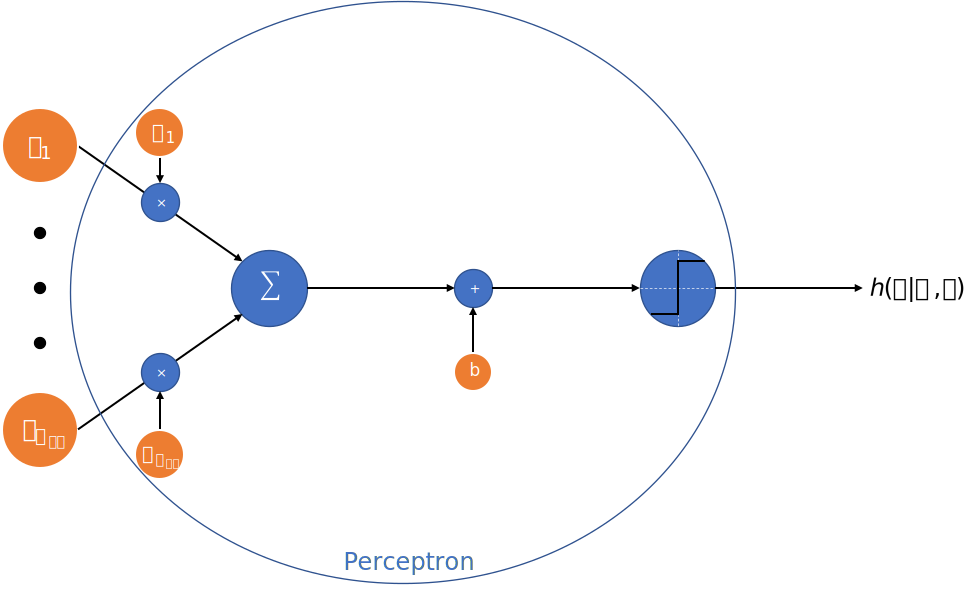
\includegraphics[width=\textwidth]{perceptron.pdf}
    \caption{The Perceptron}
    \label{fig:perceptron}
\end{figure}

%%%
    \subsection{Fully Connected} \label{subs:fcl}
    \subsection{Fully Connected layer} \label{subs:fcl}
The perceptron of Section \ref{subs:perceptron} can be considered as a linear classifier for which the decision boundary is the hyperplane, as seen in equation \eqref{eq:linearclassifer}.
%
\begin{equation}
    b + w_1 \cdot x_1 + ... + w_{n_{in}} \cdot x_{n_{in}} = 0
    \label{eq:linearclassifer}
\end{equation}
%
We can understand why the perceptron is limited because it has only a linear decision boundary. For example, we can implement the AND and OR Boolean functions using a perceptron, but it is impossible to learn the XOR function. To have a non-linear model, we must use a topology of perceptrons. This topology is composed of layers of perceptrons, where each layer, in the case of a \acrshort{cnn}, is called a \textbf{fully-connected layer}. We can see an example in Figure \ref{fig:fcn}.
%
\begin{figure}
    \centering
    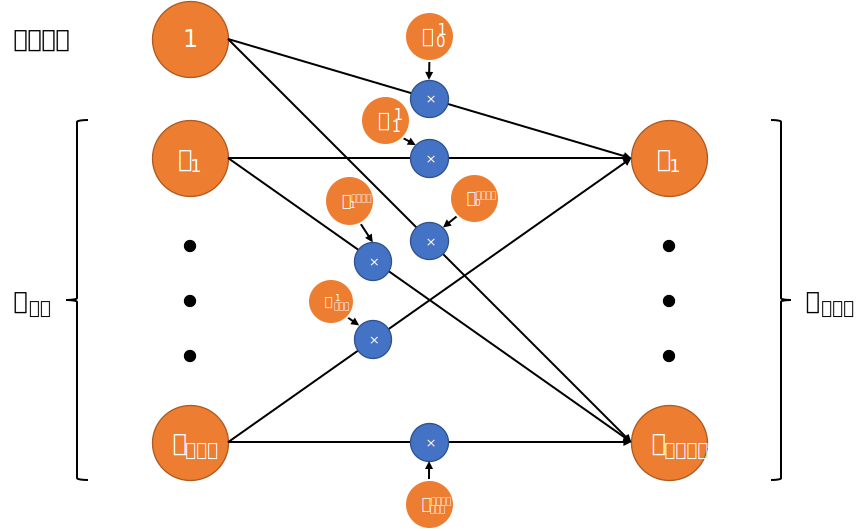
\includegraphics[width=\textwidth]{fcl.pdf}
    \caption{A fully connected layer}
    \label{fig:fcn}
\end{figure}

In the fully-connected layer, each neuron is connected to all the inputs or neurons of previous layers (as the name suggests). As the fully-connected layers are best to make a non-linear classification, we can feed those layers with extracted features, converted as a one-dimension vector \cite{khan_survey_2020}. As a result, usually, the fully-connected layers are placed at the end of \acrshort{cnn}s, where the first layers extract features from the input.

A fully-connected layer is characterized by the number of neurons, activation functions, and the values of weights. The output vector $\boldsymbol{y}$ can be expressed using equation \eqref{eq:fcn}, where $\boldsymbol{x}$ is the vector of the input of the layer and $x_0 = 1$ is the bias;   $\boldsymbol{w}$ is the vector of all the weights of the layer ($w^i_*$ are the weights of the ith perceptron and $w^*_0$ are the biases); $h$ is the activation function of the layer.
%
\begin{equation}
    \boldsymbol{y} = h(\boldsymbol{w}^T \boldsymbol{x}) \qquad \Leftrightarrow \qquad \forall o \in \{ 1, ..., N_{out} \} : y_o = h(\sum^{N_{in}}_{i=0} w^o_i \cdot x_i)
    \label{eq:fcn}
\end{equation}
%
As we have seen that perceptrons can be used to construct a non-linear classifier, we see in the next section \ref{subs:2dconv} the main operation in the \acrshort{cnn}: the \textbf{convolution}, which extracts the feature from input images.

%%%
\subsection{2D Convolution} \label{subs:2dconv}
blabla
%%%
\subsection{\acrlong{dsc}}  \label{subs:dsc}
blabla
%%%
\subsection{Bottleneck Convolution}
blabla
%%%
\subsection{Activation} \label{subs:acti}
blabla
%%%
\subsection{Pooling}
blabla
%%%%%%%%%%%%%%%%
\section{Training}
blabla
%%%%%%%%%%%%%%%%
\section{Models}
blabla
\subsection{\acrlong{dsc}}  \label{subs:mbv2}
blabla
%%%
\subsection{Pruning}
blabla
%%%
\subsection{Quantification}
blabla
